% Канонический TikZ-рисунок варианта 15. Править только здесь.
\long\def\figStereoV15{%
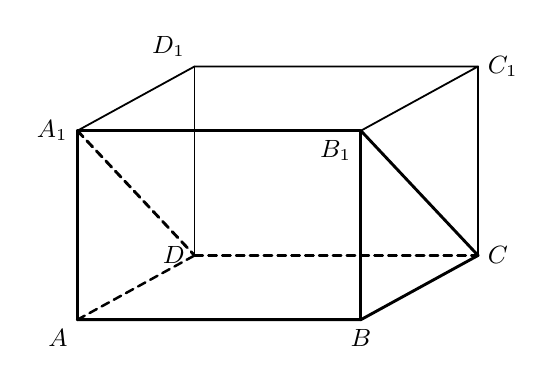
\begin{tikzpicture}[
    x={(1cm,0cm)},
    y={(0.62cm,0.34cm)},
    z={(0cm,1cm)},
    scale=0.8,
    line cap=round,
    line join=round,
    cube/.style={
        line width=0.65pt
    },
    hidden/.style={
        line width=0.65pt,
        dashed,
        dash pattern=on 3pt off 2pt
    },
    solid/.style={
        line width=1.05pt
    },
    solidhidden/.style={
        line width=0.9pt,
        dashed,
        dash pattern=on 3pt off 2pt
    },
    every node/.style={
        font=\small
    }
]

% =================================================
% Вершины прямоугольного параллелепипеда
% =================================================

\coordinate (A)  at (0,0,0);
\coordinate (B)  at (4.5,0,0);
\coordinate (C)  at (4.5,3,0);
\coordinate (D)  at (0,3,0);

\coordinate (A1) at (0,0,3);
\coordinate (B1) at (4.5,0,3);
\coordinate (C1) at (4.5,3,3);
\coordinate (D1) at (0,3,3);

% =================================================
% Рёбра исходного параллелепипеда,
% которые не входят в искомый многогранник
% =================================================

\draw[cube] (A1)--(D1)--(C1)--(B1);
\draw[cube] (D1)--(D);
\draw[cube] (C1)--(C);

% =================================================
% Скрытые рёбра искомого многогранника
% =================================================

\draw[solidhidden] (A)--(D);
\draw[solidhidden] (D)--(C);

% =================================================
% Видимые рёбра искомого многогранника
% =================================================

% Нижняя грань ABCD
\draw[solid] (A)--(B)--(C);

% Прямоугольная грань ABB_1A_1
\draw[solid] (A)--(A1)--(B1)--(B);

% Наклонная грань A_1B_1CD
\draw[hidden,solid] (A1)--(D);
\draw[solid] (B1)--(C);

% =================================================
% Подписи вершин
% =================================================

\node[below left]  at (A)  {$A$};
\node[below]       at (B)  {$B$};
\node[right]       at (C)  {$C$};
\node[left]        at (D)  {$D$};

\node[left]        at (A1) {$A_1$};
\node[below left] at (B1) {$B_1$};
\node[right]       at (C1) {$C_1$};
\node[above left]  at (D1) {$D_1$};

\end{tikzpicture}
}
